\chapter{Zbieranie i przetwarzanie danych z~czujników}
\section{Raspberry Pi}
Wszystkie zestawy zbudowano w~oparciu o~Raspberry Pi 3 v1.2. Zdecydowano się na to rozwiązanie, ponieważ bazuje na dystrybucji Linuxa, posiada opowiednie interfejsy i~złącza, a~także zintegrowany moduł WiFi. Minusem w~stosunku do konkurencyjnego Arduino jest brak wejść analogowych. Problem rozwiązano dodając zewnętrzny przetwornik A/C. Całość zamknięto w~małą plastikową obudowę z~wyciętymi otworami na czujniki (rys. \ref{the_guard_set}). Schemat budowy układu wykonano w~programie Fritzing (rys. \ref{the_guard_schem}).
\begin{figure}[H]
	\centering
	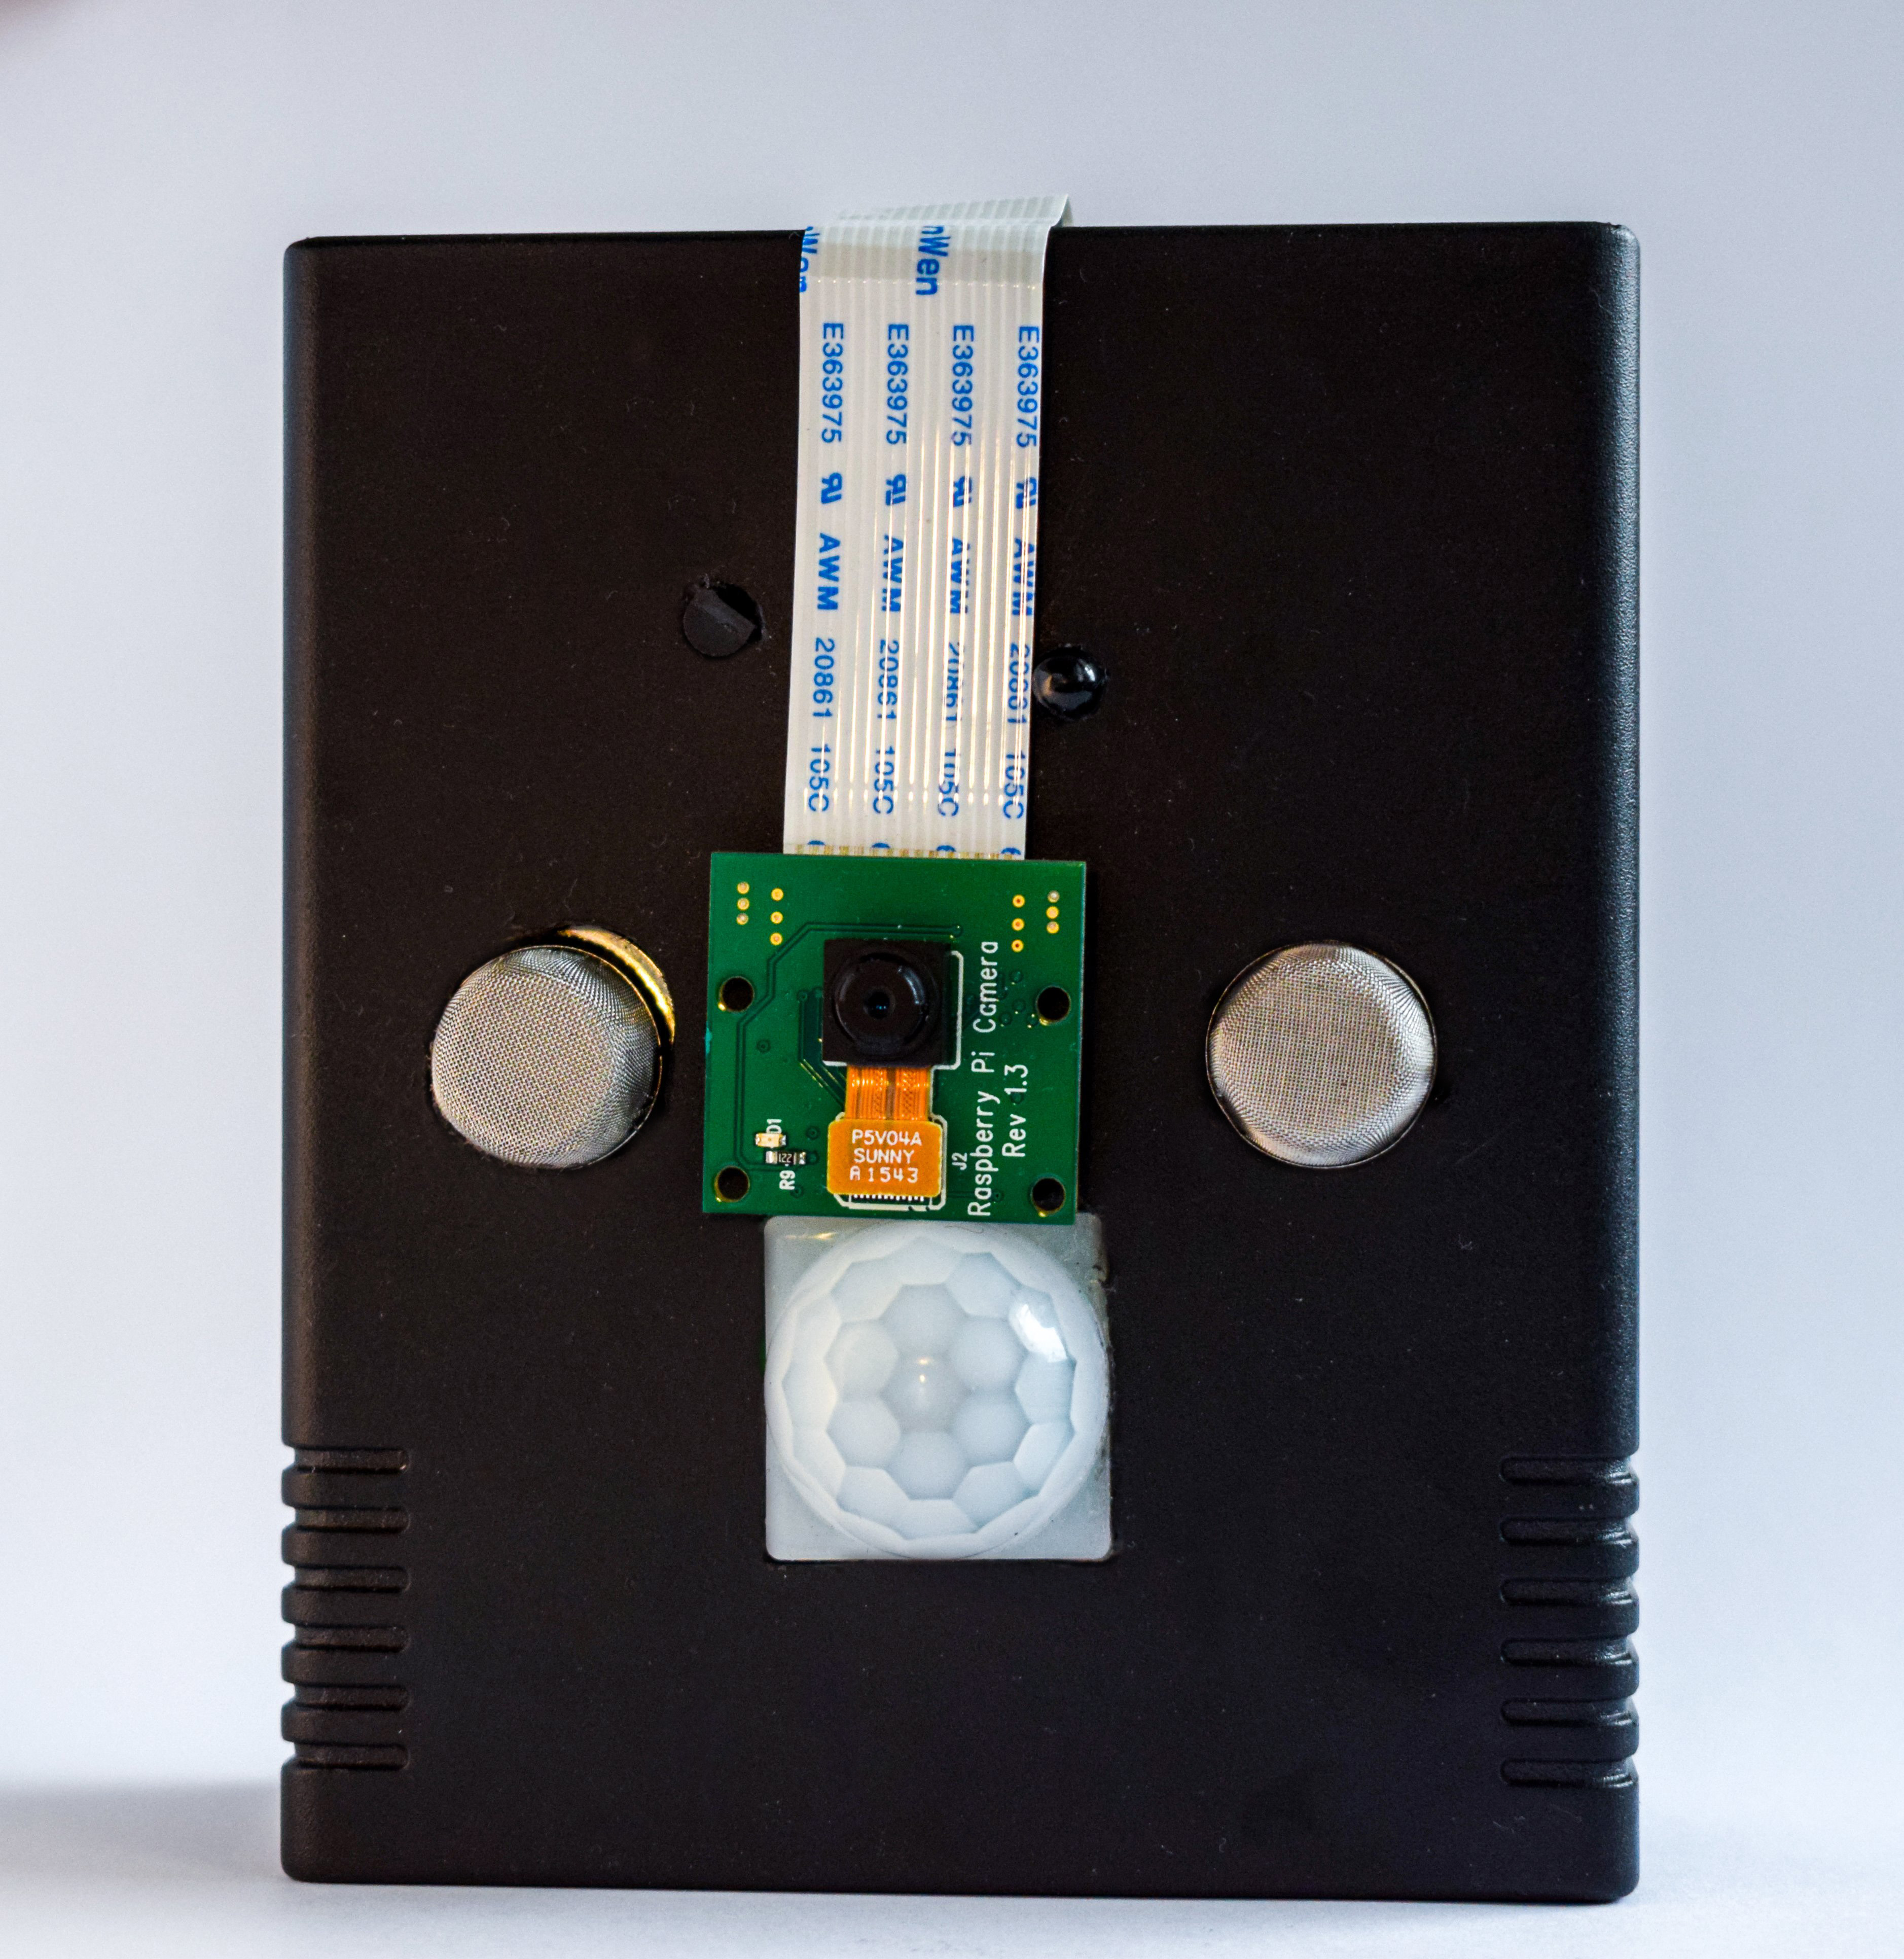
\includegraphics[width=7cm]{guard.jpg}
	\caption{Zbudowany zestaw The Guard [opracowanie własne]}
	\label{the_guard_set}
\end{figure}
\begin{figure}[H]
	\centering
	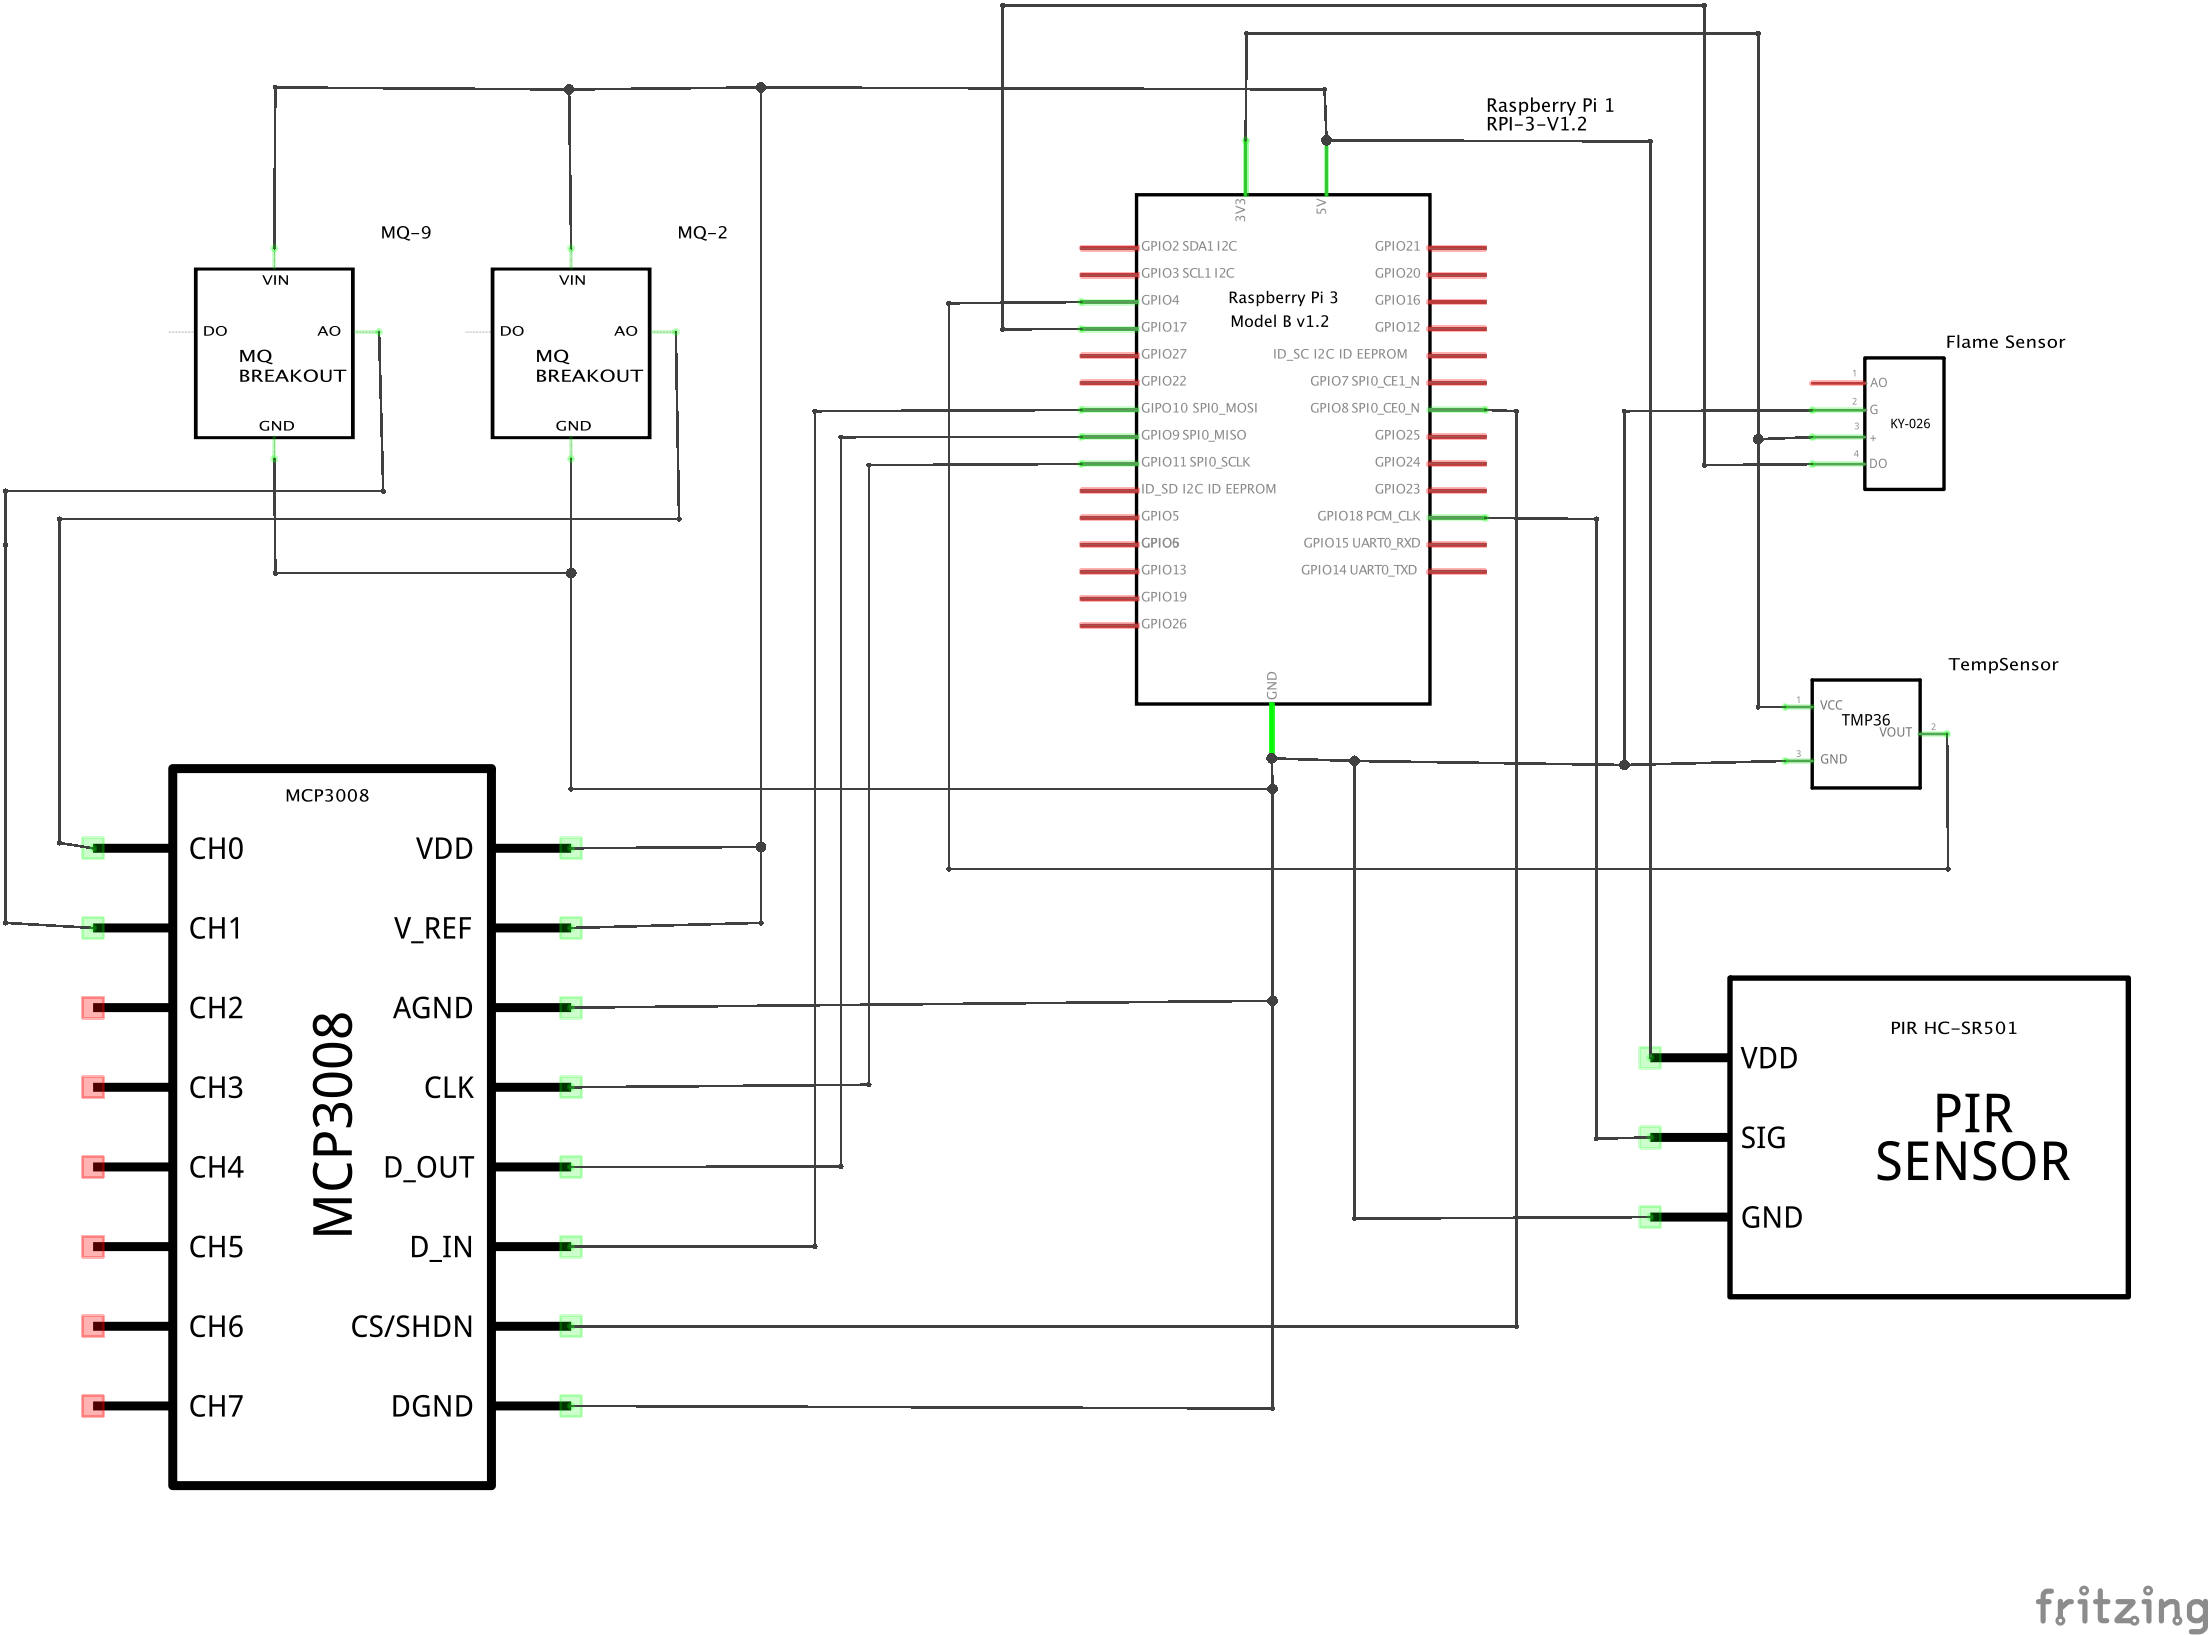
\includegraphics[width=15cm]{GuardSchem}
	\caption{Schemat układu The Guard [opracowanie własne]}
	\label{the_guard_schem}
\end{figure}
\paragraph{Specyfikacja Raspberry Pi 3 na podstawie strony Botland.com.pl \cite{specyfikacja_rasp}.}
\begin{itemize} 
\item Procesor 1.2 GHz
\item Liczba rdzeni 4. Quad Core
\item Pamięć RAM 1 GB
\item Karta pamięci microSD (w~użytych w~tej pracy urządzeniach posłużono się kartami o wielkości 8 i~16 GB).
\item 40 GPIO
\end{itemize}
Aby przygotować dowolne urządzenie Raspberry~Pi~3 do poprawnej instalacji oprogramowania The Guard należy wykonać poniższe czynności w~terminalu.
\begin{enumerate} 
\item sudo apt-get install libx264-dev
\item cd /usr/src
\item git clone git://source.ffmpeg.org/ffmpeg.git
\item sudo ./configure --arch=armel --target-os=linux --enable-gpl --enable-libx264 --enable-nonfree
\item sudo make
\item sudo install
\item sudo nano /boot/config.txt
\item w pliku config.txt dopisać Dtoverlay=w1-gpio i Gpiopin=4
\item pip intall wiringpi
\item sudo pip install spidev
\item pip install pyrebase
\end{enumerate}
Następnym krokiem jest włączenie odpowiednich interfejsów w~panelu konfiguracyjnym. Należy zmienić ustawienia zgodnie ze schematem (rys. \ref{rs_settings}).
\begin{figure}[H]
	\centering
	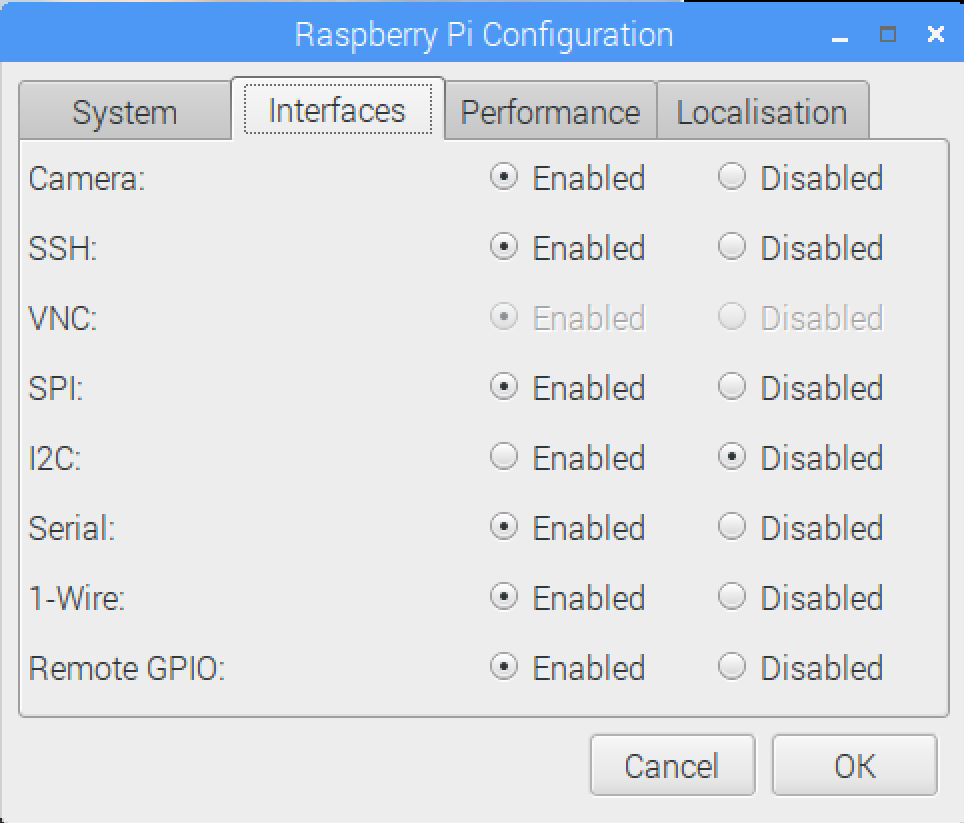
\includegraphics[width=6cm]{RSettings}
	\caption{Ustawienia [opracowanie własne]}
	\label{rs_settings}
\end{figure}
Do odczytu danych z~układów cyfrowych użyto biblioteki wiringPi. Należy podkreślić, że numeracja fizycznych pinów(rys. \ref{gpio}) i~numeracja pinów w wiringPi(rys. \ref{wiringpi}) jest różna oraz biblioteka wiringPi nie obsługuje wszystkich pinów urządzenia. Przykładowo odczyt pinu numer~1~w~wiringPi jest równoznaczny z~odczytem stanu pinu numer 12 (GPIO18).
\begin{figure}[H]
    \centering
    \subfloat[GPIO]{
	    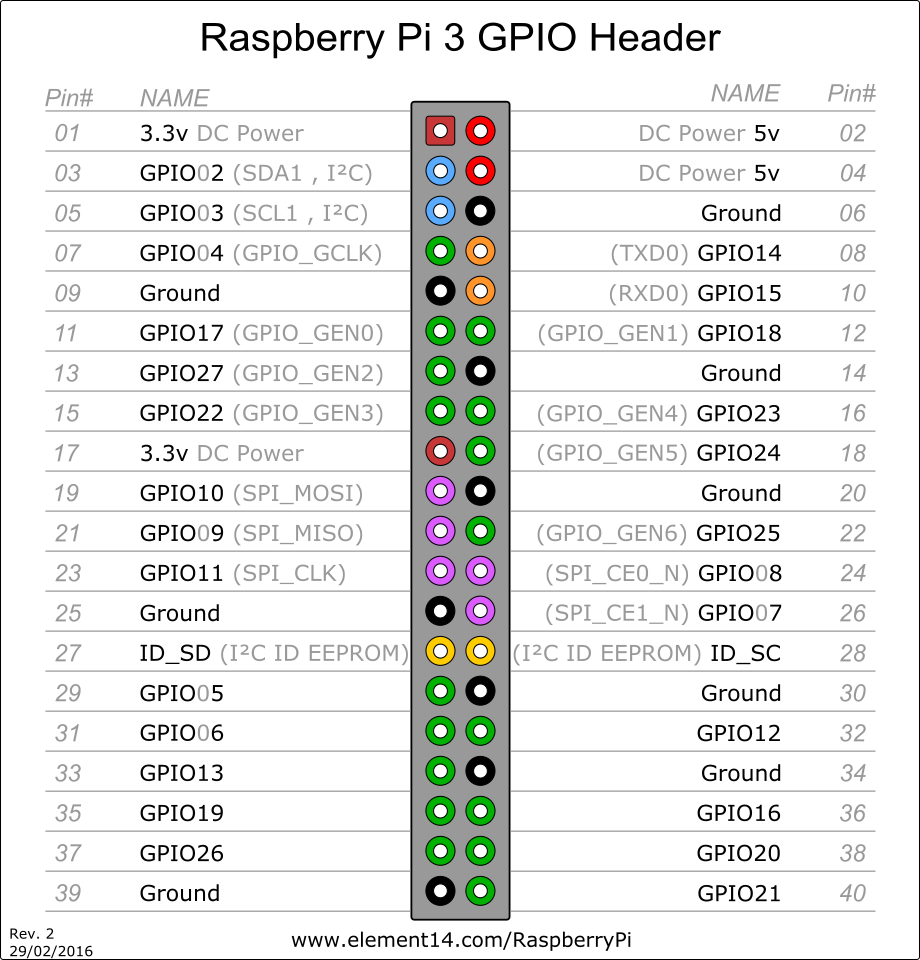
\includegraphics[width=5cm]{gpio.png}
	    \label{gpio}
	}
    \hspace{3cm} 
    \subfloat[WiringPi]{
	    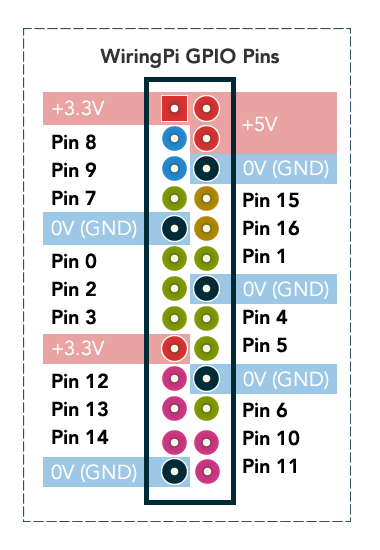
\includegraphics[height=5cm]{wiringpi.png}
	    \label{wiringpi}
	    }
    \caption{Porównanie pinów Raspberry Pi 3 \cite{gpio} z pinami wiringPi \cite{wiringpi}}
    \label{piny}
\end{figure}

Zainstalowane oprogramowanie odpowiedzialne jest za ciągłe monitorowanie stanów i~zbieranie danych z~czujników pomiarowych. Po podłączeniu układu do zasilania program jest uruchamiany automatycznie. Pierwszą czynnością jaką wykonuje Raspberry Pi jest wysłanie swojego numeru seryjnego do bazy danych Firebase. Cały proces jest w~pełni zautomatyzowany. Dzięki temu użytkownicy od razu mogą dodać urządzenie i~przeglądać dane z~czujników na aplikacjach klienckich. Dodanie akcesorium pomiarowego następuje poprzez wprowadzenie w~aplikacji jego numeru seryjnego.
\section{Czujniki}
Każdy zestaw składa się z~5~czujników, jednej kamery oraz jednego przetwornika analogowo-cyfrowego (AC). 
\paragraph{a) Specyfikacja MQ-9 - czujnik tlenku węgla \cite{specyfikacjaMQ-9}.}
\begin{itemize} 
\item Zasilanie: 5~V
\item Pobór prądu: 150 mA
\item Temperatura pracy: od -10 do 50 \textdegree{}C
\item Wyjścia: analogowe oraz cyfrowe (do pomiarów użyto wyjścia analogowego)
\end{itemize}
\paragraph{b) Specyfikacja MQ-2 - czujnik LPG i dymu \protect\cite{specyfikacjaMQ-2}.}
\begin{itemize} 
\item Zasilanie: 5~V
\item Pobór prądu: 150 mA
\item Temperatura pracy: od -10 do 50 \textdegree{}C
\item Wyjścia: analogowe oraz cyfrowe (do pomiarów użyto wyjścia analogowego)
\end{itemize}
\paragraph{c) Specyfikacja czujnika wykrywania płomieni \protect\cite{specyfikacjaFlame}.}
\begin{itemize} 
\item Zasilanie: 3.3 V
\item Zakres wykrywanej fali: 760 do 1100nm
\item Kąt detekcji: od 0 do 60 stopni
\item Temperatura pracy: od -25 do 85 \textdegree{}C
\end{itemize}
\paragraph{d) Specyfikacja DS18B20 - czujnik temperatury \protect\cite{specyfikacjaTemp}.}
\begin{itemize} 
\item Zasilanie: 3.3 V
\item Zakres pomiarowy: od -55 do 125 \textdegree{}C
\end{itemize}
\paragraph{e) Kamera:}
\begin{itemize} 
\item Wykorzystano moduł kamery Raspberry Pi
\item Kamera 5MP - wspierająca nagrywanie 30 klatek na sekundę w rozdzielczości Full HD
\end{itemize}
\paragraph{f) Specyfikacja MCP3008 - przetwornik A/C \protect\cite{specyfikacjaAC}.}
\begin{itemize} 
\item Zasilanie: od 2.7V do 5.5V
\item Pobór prądu: 0.5 mA
\item Interfejs komunikacyjny: SPI
\item Liczba kanałów: 8
\item Rozdzielczość: 10bit
\end{itemize}
\paragraph{g) Specyfikacja czujnika ruchu PIR HC-SR501 \protect\cite{pir}.}
\begin{itemize} 
\item Zasilanie: od 4.5V do 20V
\item Pobór prądu w stanie czuwania: 50 uA
\item Zakres pomiarowy: maks. 7 m
\item Kąt widzenia: do 100\textdegree{}
\end{itemize}
Na wykresach (rys. \ref{mq2}, rys. \ref{mq9}) przedstawiono charakterystyki czułości czujników MQ-2 i MQ-9.
\begin{figure}[ht]
	\centering
	\subfloat[Charakterystyka czujnika MQ-2 \protect\cite{mq2}]{
	    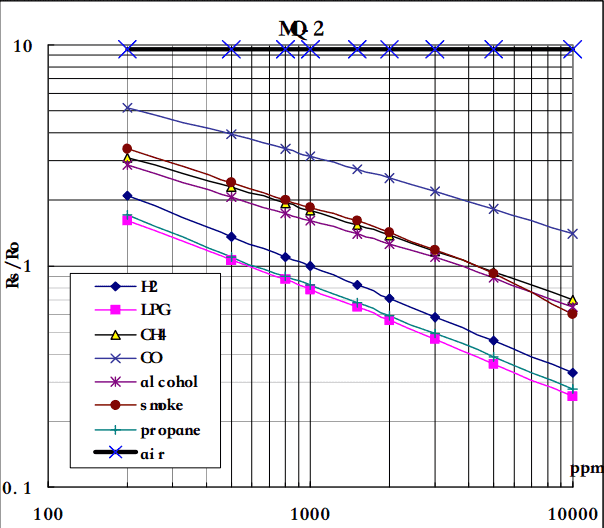
\includegraphics[height=6cm]{MQ2}
	    \label{mq2}
	}
	\hfill
	\subfloat[Charakterystyka czujnika MQ-9 \protect\cite{mq9}]{
	    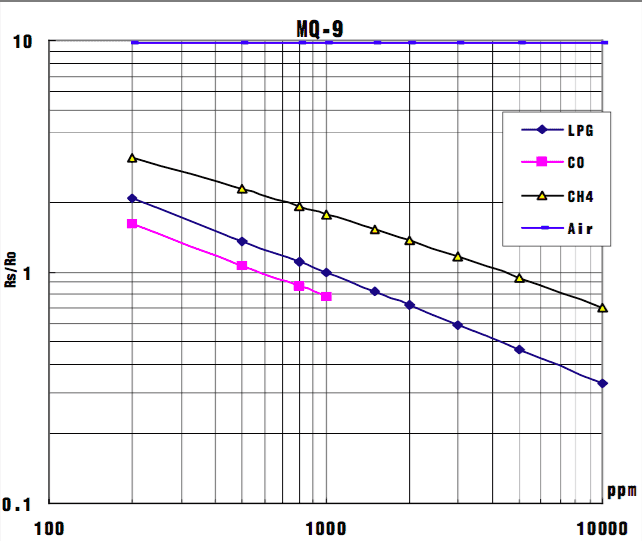
\includegraphics[height=6cm]{MQ9}
	    \label{mq9}
	    }
	\caption{Charakterystyka czujników MQ-2 oraz MQ-9.}
	\label{mq2_mq9}
\end{figure}
\\Ro - jest to stała wartość oporu czujnika przy 1000ppm H2 w~czystym powietrzu.\\
Rs - jest to opór czujnika w~różnych stężeniach gazu. \\
Przy założeniu stałej wartości Ro, przy wzroście Rs czułość czujnika maleje -~im mniejszy stosunek Rs do Ro tym dokładniejszy pomiar wykonywany przez czujnik. Na schemacie \ref{mq2_mq9} widać, że obydwa czujniki reagują na wiele różnych gazów. MQ-2 nazwano w tej pracy czujnikiem LPG, a~MQ-9 czujnikiem CO ze względu na to, że w~stosunku do tych gazów mają najwyższą czułość. 

Żaden z modeli Raspberry nie posiada wbudowanego przetwornika analogowo-cyfrowego dlatego konieczne było użycie układu zewnętrznego. Wybrano przetwornik MCP3008 ze względu na jego niski koszt i~komunikację poprzez interfejs SPI, który jest wspierany przez Raspberry Pi. MCP3008 to 10-bitowy przetwornik analogowo-cyfrowy zasilany napięciem 5V.  Przetwornik 10-bitowy jest w~stanie rozróżnić 1024 stany. Posiada 8 kanałów jednak w~projekcie wykorzystano tylko 2~–~dla MQ-9 i~MQ-2.
\paragraph{Interfejs SPI:}
\begin{figure}[ht]
	\centering
	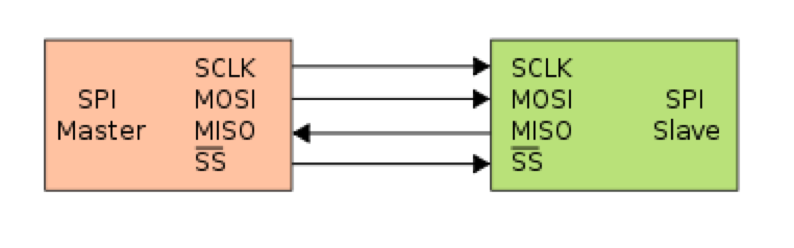
\includegraphics[width=7cm]{SPI.png}
	\caption{Interfejs SPI \protect\cite{spi}}
	\label{spi}
\end{figure}
SPI jest to interfejs synchroniczny (rys. \ref{spi}). Może być do niego podłączone wiele urządzeń typu Slave, jednak są połączone tylko z~jednym urządzeniem Master, które generuje sygnał zegarowy. Urządzenie typu Master poprzez linię SS wybiera urządzenie z~którym chce się komunikować. \\
Interfejs SPI zawiera jeszcze 3~linie.
\begin{enumerate} 
\item MOSI (ang. Master Output Slave Input). \\
Poprzez tę linię wysyłane są dane z~Raspberry Pi do przetwornika analogowo cyfrowego MCP3008.
\item MISO (ang. Master Input Slave Output).\\
Poprzez tę linię wysyłane są dane z~przetwornika AC do układu Master, czyli w~naszym przypadku Raspberry~Pi~3.
\item SCLK (ang. Serial Clock).\\
Ta linia wykorzystywana jest do przesłania zegara wygenerowanego przez Rapberry~Pi~3.
\end{enumerate}
Do komunikacji poprzez ten interfejs wykorzystano bibliotekę SpiDev \cite{spidev}. \\
Każdy układ monitoruje wskaźniki pomiarowe z czujników analogowych i~cyfrowych. W~przypadku wykrycia wskazań, które w~znaczący sposób odbiegają od normy informuje właściciela o~zagrożeniu. Informacja ta wysyłana jest do wszystkich urządzeń(smartfony, tablety itp), które posiada właściciel.  Analizując dane z~czujników analogowych w~czystym powietrzu, które wynoszą odpowiednio:\\
czujnik MQ-9: od 0.15 do 0.2,\\
czujnik MQ-2: od 0.05 do 0.15,\\
przyjęto, że granicą wysłania notyfikacji do użytkownika jest przekroczenie progu 0.3. Wartości te to znormalizowane dane z~przetwornika AC, który jak już wcześniej wspomniano wykrywa 1024 stany. Odczytywane wartości bezpośrednio na wyjściu przetwornika MCP3008 dla czujnika MQ-9 w~czystym powietrzu to około 170. Stąd 170/1024 = 0.166. Wysłanie notyfikacji wiąże się z~otrzymaniem wartości większej niż 308.

Czujniki cyfrowe wykorzystane w~pracy informują o~wykryciu płomieni lub ruchu. Czujnik ruchu wykrycie zagrożenia określa przez stan wysoki, natomiast czujnik płomieni przez stan niski. Przy implementacji zanegowano sygnał odbierany z~czujnika płomieni, aby stan wysoki zawsze informował o~niebezpieczeństwie, a~stan niski reprezentował jego brak. Na czujnikach znajduje się potencjometr, za pomocą którego dowolnie można ustawiać jego czułość. Odczyt danych następuje nieprzerwanie co 2~sekundy. Nie należy obawiać się, że aplikacja nie odczyta zagrożenia z~powodu zbyt krótkiego trwania sygnału wysokiego w bazie danych, ponieważ czujnik utrzymuje stan wysoki przez 5~sekund po wykryciu ruchu. 

Oprogramowanie wysyła także informacje z~czujników do bazy danych Firebase. Zastosowanie takiej bazy daje możliwość monitorowania wszystkich danych w~czasie rzeczywistym na aplikacjach klienckich. Dodatkowo w~przypadku zagrożenia czyli przekroczeniu progu, o~którym mowa wyżej wysyłana jest push notyfikacja do urządzeń użytkownika, a~informacja o~zagrożeniu zapisywana jest w~bazie danych Django. Każdy użytkownik jest w~stanie odtworzyć całą historię wydarzeń w~swoim systemie.

Aby zapewnić wydajny i~pewny system bezpieczeństwa przy otrzymaniu wysokich wartości na czujnikach zapisywany jest czas zdarzenia. Każda kolejna notyfikacja zostanie wysłana po upływie 10 minut od poprzedniej przy założeniu, że stan na czujniku nadal jest wysoki. 

\section{Obsługa wideo}

\paragraph{Protokół RTMP}
Podstawą funkcji strumieniowania wideo jest protokół RTMP (ang. Real-Time Message Protocol). Jest to oparty na protokole TCP protokół wysyłania obrazu, dźwięku oraz danych. \cite{MOBILERTMP}
Podstawową jednostką danych w~protokole RTMP jest wiadomość (ang. Message), której struktura jest zależna od typu strumieniowanych informacji. 
Wiadomości dzielone są na części (ang. Chunks), które są gotowe do transmisji. Strumień RTMP to ostatecznie strumień fragmentów wiadomości (ang. Chunk Stream) \cite{STREAMRTMP}.

Ponadto wykorzystano protokół HLS (HTTP Live Streaming), którego cechą jest zapisywanie odbieranego obrazu w plikach o~określonej długości. Gdy aplikacja kliencka odtwarza strumień wideo, w~rzeczywistości odbiera strumieniowane po kolei zapisane pliki .ts. Zaletą takiego rozwiązania jest płynność odbieranego wideo, a~jego wadą opóźnienie w~transmisji.

\paragraph{H264}
W~pracy wykorzystano kodowanie obrazu zgodnie ze standardem H.264. Charakteryzuje go niska złożoność algorytmów kompresji oraz niewielkie opóźnienie dzięki czemu idealnie nadaje się do zadań związanych z~szybkim enkodowaniem obrazu przed wysłaniem. \cite{H264}
Cechą charakterystyczną dla tego typu kodowania wideo jest użycie klatki kluczowej (ang keyframe, i-frame). Jest to pełna klatka obrazu, podczas gdy następujące po niej dane wyrażają różnice między dwoma tą a~następnymi klatkami. Rozwiązanie to pozwala to na zmniejszenie rozmiarów ostatecznego obrazu wideo.

\paragraph{Raspberry Pi}
Do obsługi odbioru strumienia wideo po stronie Raspberry Pi wykorzystywane jest narzędzie ffmpeg, które pozwala na przechwytywanie obrazu z kamery, ustawianie własności wysyłanego obrazu oraz punktu docelowego na który ten obraz będzie przesłany.

Pobranie numeru seryjnego urządzenia i użycie go, jako fragment adresu końcowego, gwarantuje stworzenie unikatowego dla każdego urządzenia adresu. Poniżej przedstawiono skrypt wykonujący wymienione zadania. Do pobrania obrazu z~kamery Raspberry pi posłużono się narzędziem raspivid. \cite{raspivid}
\begin{verbatim}
#!/bin/bash
serial_id="$(cat /proc/cpuinfo | grep Serial | cut -d ' ' -f 2)"
raspivid -o - -t 0 -fps 30 -b 1000000 | ffmpeg -re -ar 44100 -ac 2 
-acodec pcm_s16le -f s16le -i /dev/zero -f h264 -i - -vcodec copy -g 60 
-strict experimental 
-f flv rtmp://52.236.165.15:1936/camera/${serial_id}
\end{verbatim}
Pierwszą czynnością wykonywaną w~skrypcie jest otwarcie pliku /proc/cpuinfo. Następnie znajdowana jest w~nim linia, w~której znajduje się unikalny serial urządzenia. Następnie, z~wykorzystaniem potoku i~funkcji cut wartość ta zostaje przypisana do zmiennej serialid.

\begin{itemize}
\item Pierwszym przełącznikiem jest -o oraz parametr -. Oznacza to, że obraz z kamery jest wysyłany na wyjście standardowe.
\item Przełącznik -t ustawiony na 0~pozwala przekazywać obraz z~modułu kamery przez nieokrelony czas. Aby przestać pobierać wideo, należy użyć przerwania za pomocą sygnału SIGINT (obsługiwanego w terminalu skrótem klawiszowym CTRL+C).
\item Opcja -fps pozwala wskazać liczbę przechwytywanych klatek w~ciągu sekundy. Tutaj wykorzystano maksymalne możliwości wybranego modułu kamery.
\item Ostatnią opcją, wykorzystaną w~pobieraniu obrazu z kamery, jest bitrate, tzn wielkość jednostki pamięci w~której ma się znaleźć obraz przechwycony w~ciągu 1~sekundy strumienia. Ustawienie opcji -b~na 1000000 oznacza, że 1~sekunda wideo, może zajmować 125 kilobajtów pamięci. Jest to szczególnie istotna informacja w~kontekcie transmisji obrazu poza urządzenie przy wykorzystaniu łącza internetowego.
\end{itemize}

Drugim poleceniem jest wywołanie narzędzia ffmpeg. Odbiera ono za pomocą potoku przechwytywany obraz i~przekazuje go na docelowy punkt końcowy. Za jego pomocą ustalane są ostateczne opcje kodujące obraz w~trakcie transmisji.
\begin{itemize}
	\item Przełącznik -re pozwala odczytywać dane wejściowe z~oryginalną częstotliwością. (W powyższym skrypice zostają przechwycone ustawienia przełącznika narzędzia raspivid -fps 30).
\item Opcje  -ar, -ac, -acodec, -f, -strict odpowiadają kolejno za: próbkowanie dźwięku, wybór liczby kanałów, kodek audio, format dźwięku oraz wybór eksperymentalnego sposobu kodowania. Wymuszenie wykorzystania, jako wejścia strumienia dźwięku, na /dev/zero, oznacza, że strumień ten zostaje wypełniony wartościami pustymi. Zatem opcje transmisji dźwięku są nieistotne.
\item Przełącznik -vcodec ustala kodek wideo. W~pracy wykorzystano standard kodowania H.264.
\item Następnie ustawiono wejście obrazu. Przełącznik -i - powoduje, że narzędzie ffmpeg przechwytuje, dzięki potokowi, obraz przekazywany funkcją raspivid.
\item Opcja -g 60 oznacza, że tzw klatka kluczowa (ang. keyframe) pojawia się co 60 klatek (w~tej sytuacji co 2 sekundy). 
\item Przełącznik -f w~przypadku strumienia obrazu z~kamery wymusza format nadawanego wideo.  
\item Ostatnim elementem polecenia jest podanie punktu docelowego dla strumienia. Za pomocą protokołu RTMP, obługiwanego przez serwer o~adresie IP 52.236.165.15 na porcie 1936, obraz wysyłany jest na aplikację o~nazwie camera i~punkt charakteryzowany przez numer seryjny urządzenia. Działanie tego elementu opisano w kolejnym punkcie. 
\end{itemize}

\paragraph{Serwer}
Narzędziem umożliwiającym obsługę proxy jest serwer nginx. W~części projektu związanej ze strumieniowaniem wideo wykorzystano moduł nginx-rtmp \cite{NGINX}. Umożliwia on obsługę obrazu transmitowanego z~wielu źródeł, na wiele urządzeń równocześnie. 
Moduł ten pozwala na realizację wielu funkcji, a niektóre z nich przedstawiono poniżej.
\begin{itemize}
\item Tworzenie dynamicznych punktów końcowych, dla urządzeń strumieniujących obraz.
\item Zmianę parametrów przechwytywanego obrazu .
\item Zapisywanie nagrań po stronie serwera.
\item Tworzenie punktów nadających, dla aplikacji odtwarzających strumień.
\end{itemize}
Ponadto pozwala na utworzenie aplikacji HLS przechowującej tymczasowo obraz, zanim zostanie on przesłany dalej. Pozwala to na uniknięcie opóźnień między kolejnymi klatkami obrazu.

Wszystkie funkcjonalności są zdefiniowane poprzez ustawienia pliku konfiguracyjnego, którego lokalizacja to /usr/local/nginx/conf/nginx.conf:

\begin{verbatim}
rtmp {
    server {
            listen 1936;
            chunk_size 4096;
            application camera {
                    hls on;
                    hls_path /mnt/hls/;
                    hls_fragment 2;
                    hls_playlist_length 3;
                    allow publish all;
                    allow play all;
                    live on;
                    record off;
             }
    }
}
\end{verbatim}

Powyższy plik koniguracyjny powoduje, że serwer rtmp dostępny jest na porcie 1936 (domyślne porty dla protokołu RTMP na urządzeniach z~systemem z~rodziny Ubuntu to 1935 i~1936). Następnie tworzona jest aplikacja o~nazwie camera. Dla aplikacji wysyłających dane, jest ona dostępna pod adresem: rtmp://<ip-serwera>:1936/camera/<klucz>, gdzie klucz jest wybierany przez aplikację i~tworzony dynamicznie, gdy tylko urządzenie zacznie nadawać dane pod wskazany adres.
Ustawienia aplikacji decydują o~tym, że dla urządzeń odtwarzających wideo, dostępne jest ono dzięki aplikacji HLS - opcja hls on. Na szczególną uwagę zasługują linie: hls~fragment~2~oraz hls~playlist~length~3, które wskazują na to, że po stronie serwera nagrywane są 2~tymczasowe fragmenty, o~długości 3~sekund każdy. Pliki te są przechowywane w~folderze /mnt/hls/, a~ich nazwę jednoznacznie będzie wskazywać klucz strumienia.

\begin{verbatim}
http {
    server {
        listen       80;
        location /hls {
                types {
                        application/vnd.apple.mpegurl m3u8;
                        video/mp2t ts;
                }
        root /mnt/;
        }
    }
}
\end{verbatim}

Konfiguracja ta udostępnia aplikację HLS. Dla aplikacji klienckich, obraz będzie dostępny pod adresem: http://<ip-serwera>:80/hls/<klucz>.m3u8, o~czym decyduje konfiguracja części związanej z serwerem RTMP.

